\documentclass[portrait,final]{baposter}
%\documentclass[a4shrink,portrait,final]{baposter}
% Usa a4shrink for an a4 sized paper.

%\tracingstats=2

\usepackage{times}
\usepackage{calc}
\usepackage{graphicx}
\usepackage{amsmath} 
\usepackage{amssymb}
\usepackage{amsbsy} 
\usepackage{relsize}
\usepackage{multirow}
\usepackage{bm}
%\usepackage{natbib}

\usepackage{graphicx}   
\usepackage{multicol}

\usepackage{pgfbaselayers}
\pgfdeclarelayer{background}
\pgfdeclarelayer{foreground}
\pgfsetlayers{background,main,foreground} 
\usetikzlibrary{shadows}

\usepackage{helvet}
%\usepackage{bookman}
\usepackage{palatino}


\selectcolormodel{cmyk}


\begin{document}
\definecolor{lightersilver}{cmyk}{0,0,0,0.1}
\definecolor{silver}{cmyk}{0,0,0,0.3}
\definecolor{darksilver}{cmyk}{0,0,0,0.4}
\definecolor{yellow}{cmyk}{0,0,0.9,0.0}
\definecolor{reddishyellow}{cmyk}{0,0.22,1.0,0.0}
\definecolor{black}{cmyk}{0,0,0.0,1.0}
\definecolor{darkYellow}{cmyk}{0,0,1.0,0.5}
\definecolor{darkSilver}{cmyk}{0,0,0,0.1}
%\definecolor{darkSilver}{cmyk}{0,0,0,0.1}

\definecolor{lightyellow}{cmyk}{0,0,0.4,0.0}
\definecolor{lighteryellow}{cmyk}{0,0,0.1,0.0}
\definecolor{lightestyellow}{cmyk}{0,0,0.05,0.0}

\newcommand{\bs}[1]{\boldsymbol{#1}}

\begin{poster}%
{
grid=no,
colspacing=0.7em,
bgColorOne=white,%lightersilver, 
bgColorTwo=white,%lightersilver,
borderColor=reddishyellow, 
headerColorOne=yellow,
headerColorTwo=reddishyellow, 
headerFontColor=black,
boxColorOne=lightersilver,
boxColorTwo=lighteryellow,
textborder=rounded,
eyecatcher=yes,
headerborder=open,
headerheight=0.07\textheight,
headershape=rounded,
headershade=shade-tb,
headerfont=\Large\textsf, %Sans Serif
boxshade=plain, 
background=plain,
linewidth=2pt
}
  % Eye Catcher must be on to center the rest
{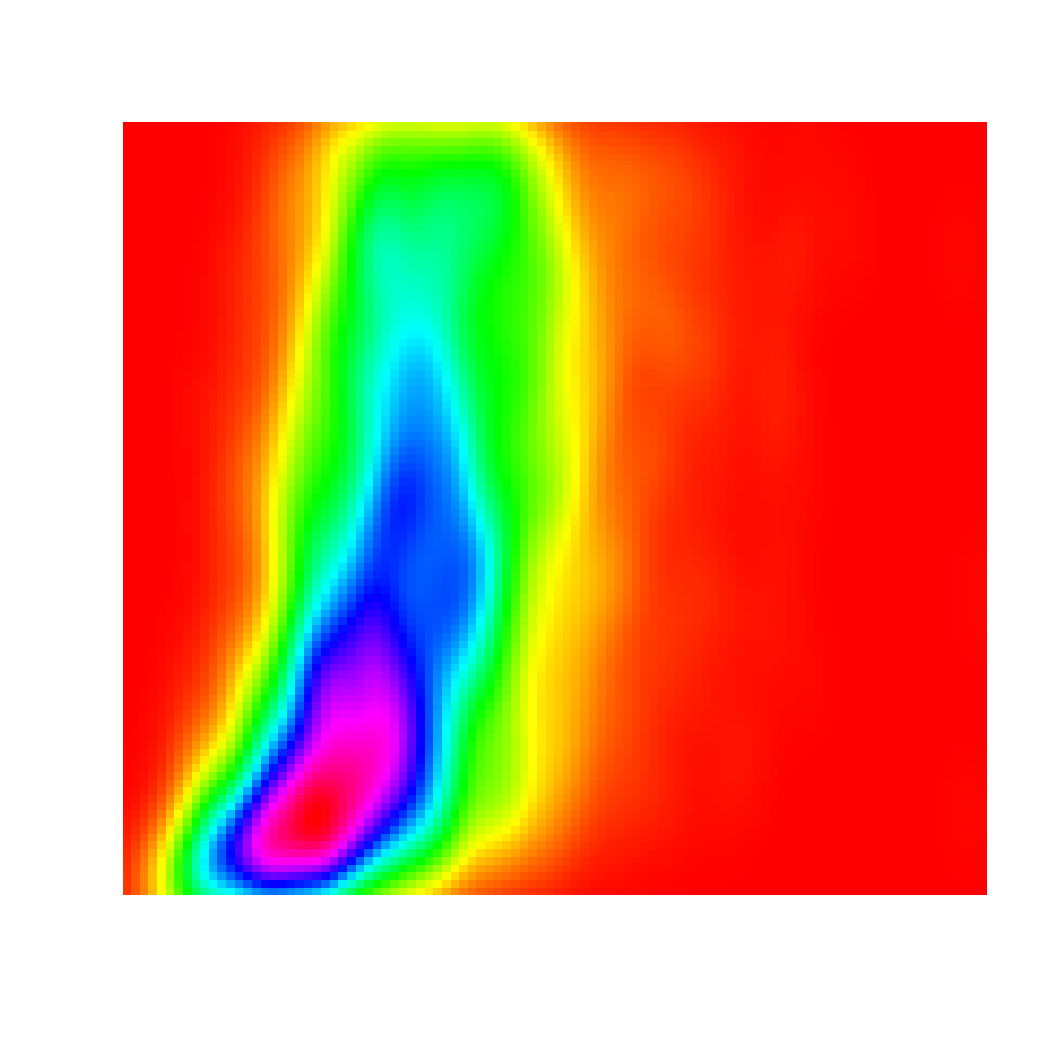
\includegraphics[height=1.9cm]{eyeCatch1.png}\hspace{.2cm} 
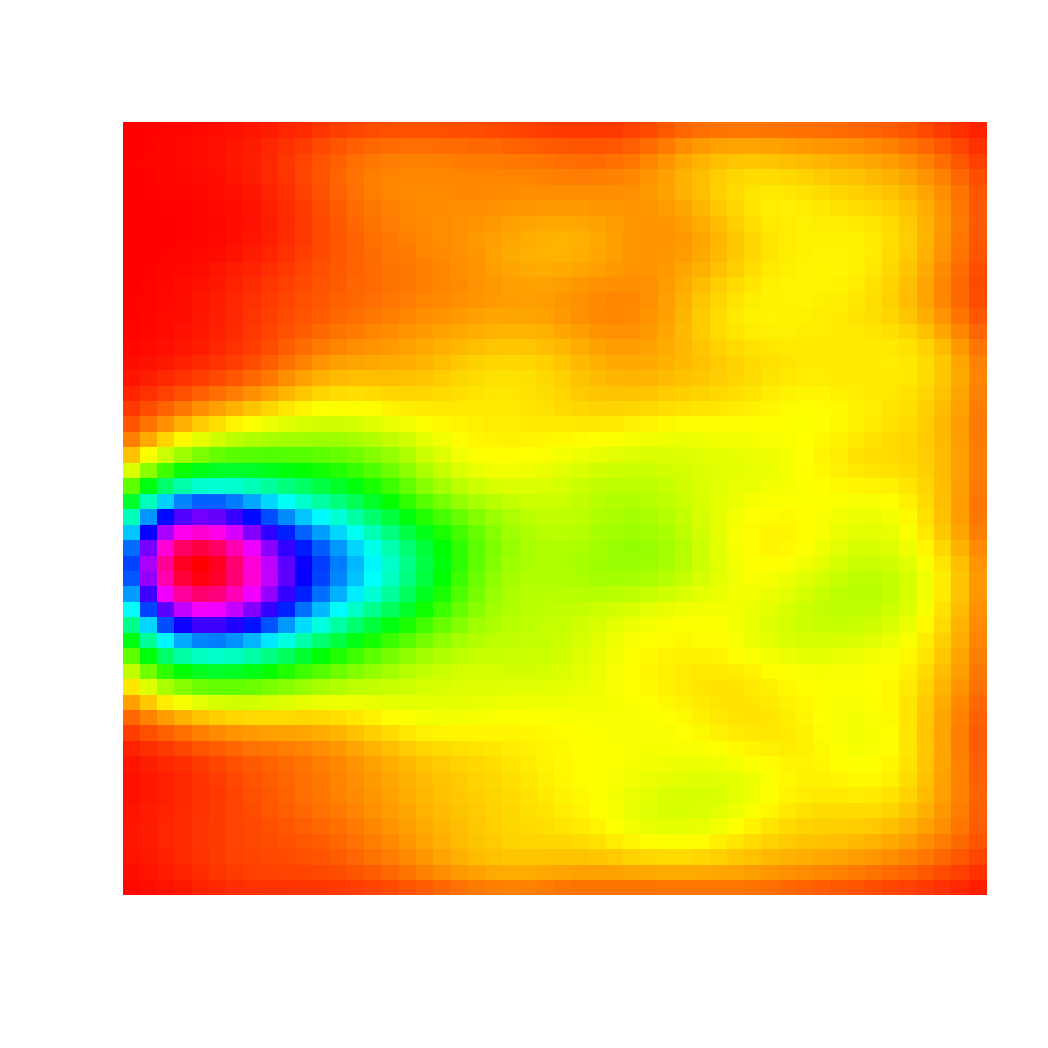
\includegraphics[height=1.9cm]{eyeCatch2.png}} 
{\sc\Huge Introducing {\it msms}}
{\sc \hspace{1cm} Gregory Ewing and Joachim Hermisson
\newline {\small http://www.mabs.at/ewing/msms/}}
{
\begin{minipage}{0.2625\textwidth}
%\begin{center}

\includegraphics[height=1cm]{uni_logo_farbe_01.pdf}
\newline
\includegraphics[height=1cm]{mfpl_logo3d_transparent.png}
%\end{center}
\end{minipage} 
}   
%%%%%%%%%%%%%%%%%%%%%%%%%%%%%%%%%%%%%%%%%%%%%%%%%%%%%%%%%%%%%%%%%%%%%%%%%%%%%%
%%% Now define the boxes that make up the poster
%%%---------------------------------------------------------------------------
%%% Each box has a name and can be placed absolutely or relatively.
%%% The only inconvenience is that you can only specify a relative position 
%%% towards an already declared box. So if you have a box attached to the 
%%% bottom, one to the top and a third one which should be in between, you 
%%% have to specify the top and bottom boxes before you specify the middle 
%%% box.
%%%%%%%%%%%%%%%%%%%%%%%%%%%%%%%%%%%%%%%%%%%%%%%%%%%%%%%%%%%%%%%%%%%%%%%%%%%%%%
 
\headerbox{Abstract}{name=abstract,column=0,row=0}{

We have implemented a coalescent simulation program for a structured population
with selection at a single diploid locus. The program includes the functionality
of the simulator {\it ms} to model population structure and demography, but adds
a model for deme- and time-dependent selection using forward simulations. The
program can be used, e.g.\, to study hard and soft selective sweeps in structured
populations or the genetic footprint of local adaptation. The implementation is
designed to be easily extendable and widely deployable. The interface and output
format are compatible with {\it ms}. Performance is comparable even with
selection included. We also discuss some applications. 
  \vspace{0.4em}
}

\headerbox{{ msmsABC}}{name=abc,column=2,row=0}{

The ability to simulate all kinds of selective scenarios efficiently opens the possibility to 
estimate selection parameters via Approximate Bayesian Computation (ABC). 
{\it msmsABC} is designed to be compatible with the ABC toolbox from
the CMPG lab at the University of Bern.

\vspace{1em}


\begin{tikzpicture}
\draw (-1.5,0) node[anchor=north west]
{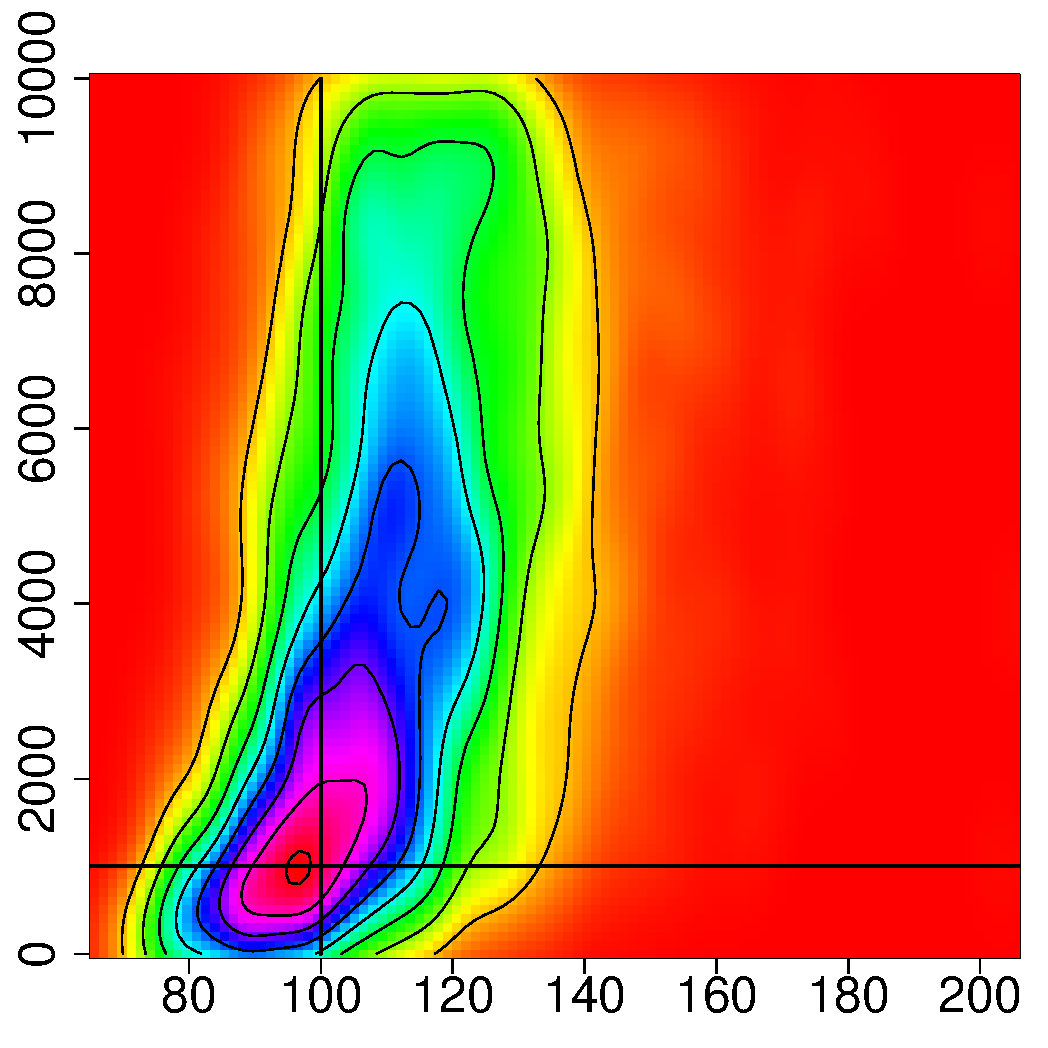
\includegraphics[width=0.8\textwidth]{2dAlphaThetaL.pdf}}
(1.5,0.1) node[above] 
{\bfseries Mutation Rate $\bs\theta$ and Selection Coefficient $\bs\alpha$}
(-1.7,-2.75) node[left] {\large $\bs\alpha$}
(1.5,-5.8) node[below] {\large $\bs\theta$};
\end{tikzpicture}

\vspace{0.5em}

The posterior density support for estimation of neutral mutation rate $\theta$
and selection strength $\alpha$. The true values fall in the 95\% confidence
interval. These results were obtained in one million simulations co-estimating
recombination rate, fixation time and the position of the selected locus. The
simulation took about 4 hours.

\vspace{1em}

\begin{tikzpicture}
\draw (-1.5,0) node[anchor=north west]
{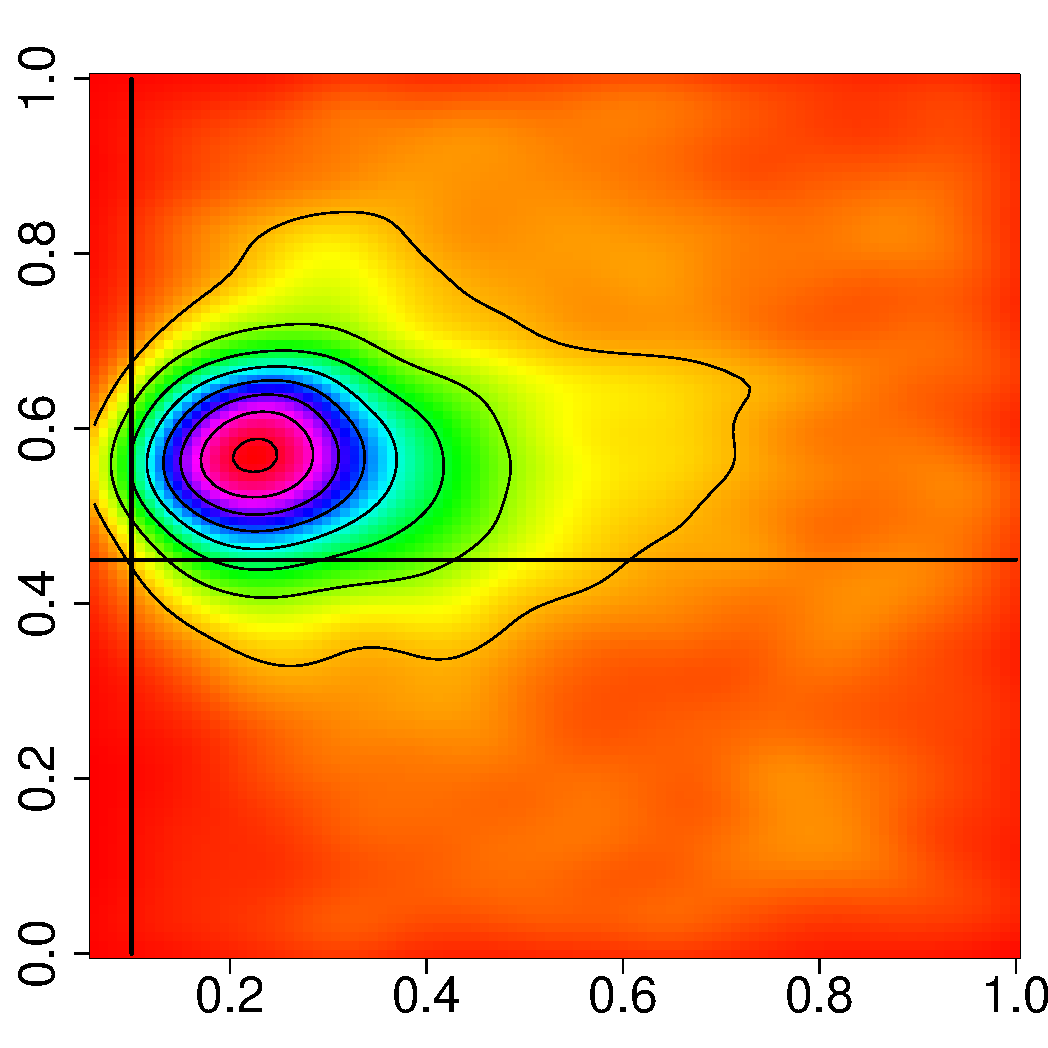
\includegraphics[width=0.8\textwidth]{2dPosTimeL.pdf}}  
(1.5,0) node[above] 
{\bfseries Position of Selected Site and Fixation Time}
(-1.7,-2.5) node[left,rotate=90] {\bfseries Position}
(1.5,-5.8) node[below] {\bfseries Fixation Time};
\end{tikzpicture}

\vspace{0.5em}

The estimation of fixation time and position of the selected locus proved to be more difficult, the 
true value was not included in the 95\% confidence interval but was still
inside the 99\% confidence interval.

However, as with all ABC methods, picking the right statistics can be difficult
and we are currently investigating statistics that are the most informative with
respect to selection parameter estimation. Thus we are confident we can improve
the estimation of fixation time and position.

\vspace{0.5em}
}

\headerbox{Conclusion}
 {name=theend,below=abc,span=1,column=2}{
 
 {\it MSMS}\cite{ewing2010} is a powerful coalescent simulator with selection
 at a single locus. It is fast and compatible with {\it ms} which permits easy extension of
 existing {\it ms} pipelines to include selection. A wide range of applications
 are possible with the combination of flexibility and speed that {\it msms}
 provides. Examples include ABC frameworks, power studies and selection test
 development.  
 
 \vspace{.4em} 
 }

\headerbox{Simulations}{name=sims,below=abstract,column=0}{

{\it MSMS}\cite{ewing2010} uses an infinite sites mutation model and locus
model.
\vspace{.1cm}

\includegraphics[width=1\textwidth]{locus.pdf}

Simulations are carried out in the following steps:
\begin{enumerate}
  \item A forward pass simulates selection with drift. The
  result is the frequency of the selected allele over time for each deme.
  \item The coalescent is then simulated in the pastward direction {\em
  conditional} on the frequency of the selected locus.
  \item Neutral mutations are added to the ancestral recombination graph.
\end{enumerate}
To sample the coalescent conditionally on frequency,  we assume discrete generations 
during the selected phase. Two lineages can only be nonrecombinant
descendants of a parent if they share the allele at the selected locus. Therefore the
effective population size of the selected allele is scaled by the frequency.
All other events are affected similarly. 
\vspace{0.4em}
}

\headerbox{Performance: {\it msms } vs. {\it ms}}
{name=speed,below=sims,bottomaligned=theend,column=0}{

\begin{tikzpicture}
\draw (-1.5,0.4) node[anchor=north west]
{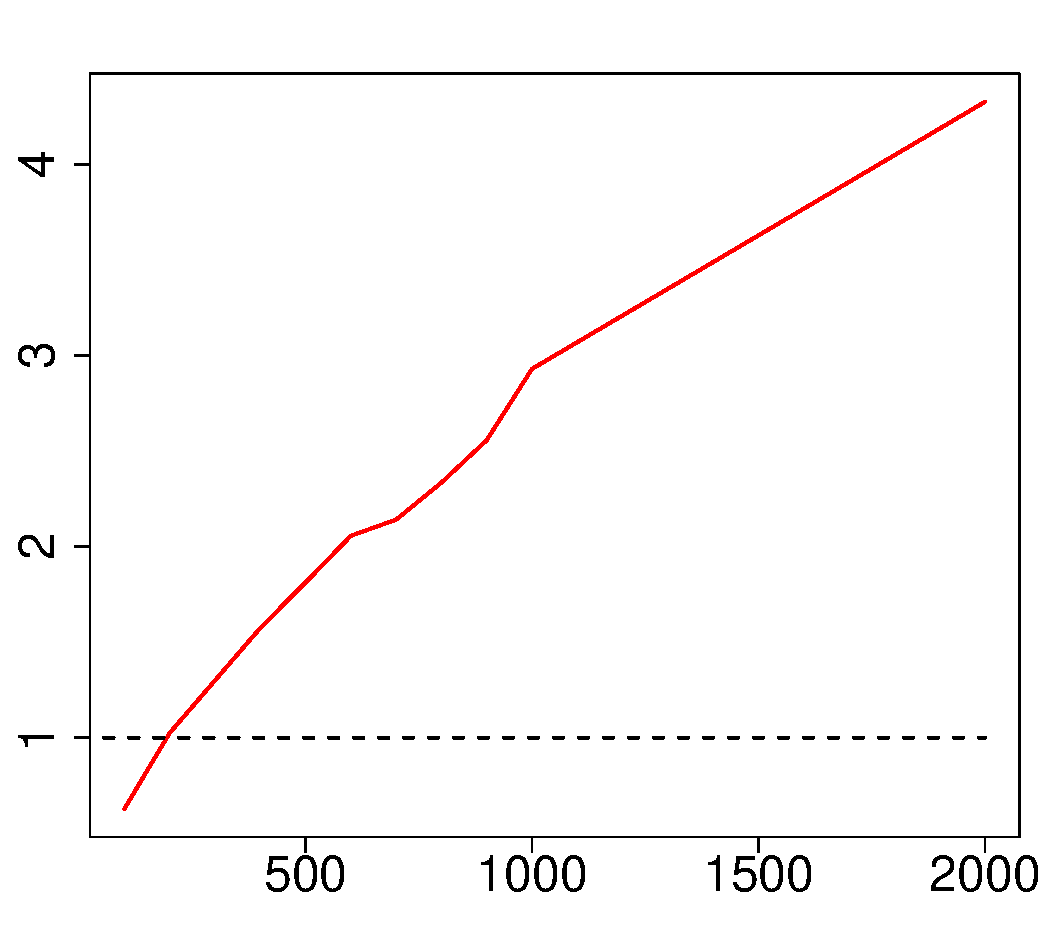
\includegraphics[width=0.8\textwidth]{fastL.pdf}}
(1.5,0) node[above] 
{\bfseries Speedup Ratio of {\it msms} vrs {\it ms}}
(-1.7,-1) node[left,rotate=90] {\bfseries Speedup Factor}
(1.5,-4.8) node[below] {\bfseries Recombination Rate $\bs\rho$};
\end{tikzpicture}

The figure shows the computing speed of {\it msms} without selection compared to
{\sc ms} on a standard desktop PC:  AMD64 X2 Dual Core Processor 6000+, using Sun
Java 1.6u18 64bit and gcc 4.2.3.
{\it msms} is faster than {\sc ms} with intermediate to high
recombination. The command line used was:

{\tt ms 50 1000 -t 100 -r $\rho$ 10000}

\vspace{0.4em}
}



\headerbox{Complex Models\hspace{-1pt} and\hspace{-1pt} Selection}
{name=example,bottomaligned=abc,column=1,row=0,span=1}{
\begin{tikzpicture}
[scale=.7]
%\draw[help lines] (0,-10) grid (10,10);
 %[stealth-stealth]
\draw [<->, line width=2pt,>=stealth] (2.5,5) -- (intersection of 2.5,5--5,5
and 4.5,4--2.5,6.5); 
\draw [<->, line width=2pt,>=stealth] (2.5,2) -- (4.33,2);
\draw [<->,>=stealth] (5,2) -- (5.5,2);
\draw [<->, line width=2pt,>=stealth] (2.5,3) -- (5.5,3);
\draw [->,line width=3pt,blue,>=stealth] (8.7,0.1) .. 
	controls (8,1.5) and (7.5,1.5) ..
	(7.2,0.1);
\draw [->,line width=3pt,red,>=stealth] 
(5.5,8.5) .. controls (7,8.5) and (8.5,2) .. (6.5,.7);
\shade[top color=blue,bottom color=blue,thick]
(0,0) -- (0,10)  --(2,10) -- (2,9) --
(2.5,9) -- (2.5,8) -- (6,4) -- (6,3.5)
.. controls (8,3.5) and (10,2) .. (10,0) 
-- (8.5,0) 
.. controls (9,1) and (8,3.2) .. (6,3.2)
.. controls (6,2.2) and (6,0) .. (8,0)
-- (5.5,0) -- (5.5,4) -- (5,4) -- (5,0) -- (3,0) 
.. controls (4.5,0) and (4.5,4) .. (4.5,4) 
-- (2.5,6.33) -- (2.5,0) -- cycle  
(9.5,-.1) node[below] {MXL(4)}
(6.5,-.1) node[below] {CEU(3)}  
(4,-.1) node[below] {CHB(2)} 
(1,-.1) node[below] {YRI(1)}
(3,9) node[right,text width=5cm] {\tt \bfseries -Smu 0.1 -SI 0.05 5 0 0 0.01  0
0 -Sc 0 3 1000 5000 0 -Sp 0.5};

\shade[top color=blue,bottom color=green]
(6,4) -- 
(6,3.2).. controls (6,2.2) and (6,0) .. (8,0)
-- (5.5,0) -- (5.5,4) ; 
%now we add pictures
\draw 
(5,-1) node[above]{Neutral}
(0,-1) node[anchor=north west]
{\includegraphics[width=\textwidth]{../applicationNote/noSelectionJAFSRange.pdf}}
(5,-5) node[above]{Selection}
(0,-5) node[anchor=north west]
{\includegraphics[width=\textwidth]{../applicationNote/selectionJAFSRange.pdf}};
\end{tikzpicture} 


{\it MSMS} can simulate selection on top of any demography that could be simulated with {\it ms} . 
As an example we picked a current model of human
demography\cite{gutenkunst_inferringjoint_2009}, that includes bottle necks, growth, migration and admixture.
In addition we simulate selection in CEU with the following command line
options:
\begin{itemize}
\item {\tt  -Smu}  advantageous mutation rate $a\to A$ of $4N_e\mu=0.1$.
Traditionally this means we would be considering a soft sweep. However in this
case we have overdominance.
\item {\tt  -SI}   start time of selection (0.05) and frequencies of the the
advantageous allele in each deme from standing genetic varaition(0.01\% in CEU).
\item {\tt  -Sc}  Overdominant selection pastward from time 0 only in CEU.
Selection coefficients: $\alpha_{AA}=1000$ $\alpha_{aA}=5000$ $\alpha_{aa}=0$. 
\item  {\tt  -Sp} position of the selected locus 

\end{itemize}

In the lower panel are heat maps of the pair-wise joint allele frequency spectra given the demography 
under neutrality and the described selection scheme.
\vspace{0.4em}
}


\headerbox{\smaller Citations and Acknowledgements}
{name=cite,below=example,column=1,bottomaligned=theend} { 
\small 

Funding from the DFG and the WWTF is gratefully acknowledged. Thanks also to
Peter Pfaffelhuber, Cornelia Borck, Ines Hellmann, Pleuni Pennings and Jayne
Ewing.

\vspace{-1.2cm}
\bibliographystyle{Science}
\renewcommand\refname{}
\bibliography{Bio}
}


\end{poster}% 
\end{document}
